\documentclass[a4paper]{article}
\usepackage[utf8]{inputenc}
\usepackage{todonotes}
\usepackage[russian]{babel}
\usepackage{graphicx}
\usepackage{float}
\usepackage{wrapfig}
\usepackage{tikz}
\usepackage{amsmath, amssymb}
\usepackage{hyperref}
\usepackage{listings}
\usepackage{caption}
\usepackage{geometry}
\usepackage{fancyhdr}
\usepackage{nicefrac}
\usepackage{xcolor}
\geometry{left=2cm,right=2cm,top=2cm,bottom=2cm}
\definecolor{urlcolor}{rgb}{0,0,1}
\hypersetup{pdfborder=0 0 0}
\hypersetup{pdfstartview=FitH, linkcolor=linkcolor, urlcolor=urlcolor, colorlinks=true}

\definecolor{strings}{rgb}{0,0.6,0}
\definecolor{comments}{rgb}{0,0.3,0}
\definecolor{numbers}{rgb}{0.5,0.5,0.5}
\definecolor{keywords}{rgb}{0.09,0.61,0.95}
\definecolor{background}{rgb}{0.97,0.97,0.97}

\lstdefinestyle{codestyle}{
    backgroundcolor=\color{background},
    commentstyle=\color{comments},
    keywordstyle=\color{keywords},
    stringstyle=\color{strings},
    numberstyle=\tiny\color{numbers},
    basicstyle=\ttfamily\footnotesize,
    breakatwhitespace=false,
    breaklines=true,
    captionpos=b,
    inputencoding=utf8,
    keepspaces=true,
    numbers=left,
    numbersep=5pt,
    showspaces=false,
    showstringspaces=false,
    showtabs=false,
    tabsize=2,
    extendedchars=true
}

\lstset{style=codestyle}

\newcommand{\addsection}[1]{
    \phantomsection
    \addcontentsline{toc}{section}{#1}
    \section*{#1}
}
\newcommand{\addsubsection}[1]{
    \phantomsection
    \addcontentsline{toc}{subsection}{#1}
    \subsection*{#1}
}
\newcommand{\addsubsubsection}[1]{
    \phantomsection
    \addcontentsline{toc}{subsubsection}{#1}
    \subsubsection*{#1}
}

\begin{document}

% Титульный лист
\begin{titlepage}
    \centering
    {\large Федеральное государственное автономное образовательное учреждение\par}
    {\large высшего образования\par}
    {\bfseries САНКТ-ПЕТЕРБУРГСКИЙ НАЦИОНАЛЬНЫЙ ИССЛЕДОВАТЕЛЬСКИЙ УНИВЕРСИТЕТ ИТМО\par}
    {\bfseries Факультет систем управления и робототехники\par}
    \vfill
    {\Large \bfseries Лабораторная работа №3\par}
    {\Large \bfseries Жесткая фильтрация\par}
    \vfill
    
    \begin{flushright}
        Студент: Сайфуллин Д.Р. \\
        Поток: ЧАСТ.МЕТ. R23 1.5 \\ 
        Преподаватели: Перегудин А.А.\\
        Догадин  Е.В.
    \end{flushright}
    \vfill
    Санкт-Петербург \\
    2025 г.
\end{titlepage}

% Оглавление
\tableofcontents
\newpage

\addsection{Задание 1. Жесткие фильтрации}
\addsubsection{Постановка задачи}
Для выполнения задания необходимо задать параметры \(a, t_1, t_2\) и рассмотреть предложенную функцию. Пусть \(a = 3, t_1 = -2, t_2 = 1\), тогда функцией нашего сигнала будет:
\[g(t)=
\begin{cases}
    3, & t \in [-2,1],\\[1ex]
    0, & \text{иначе}.
\end{cases}\]
Построим график нашей функции: 
\begin{figure}[H]
    \centering
    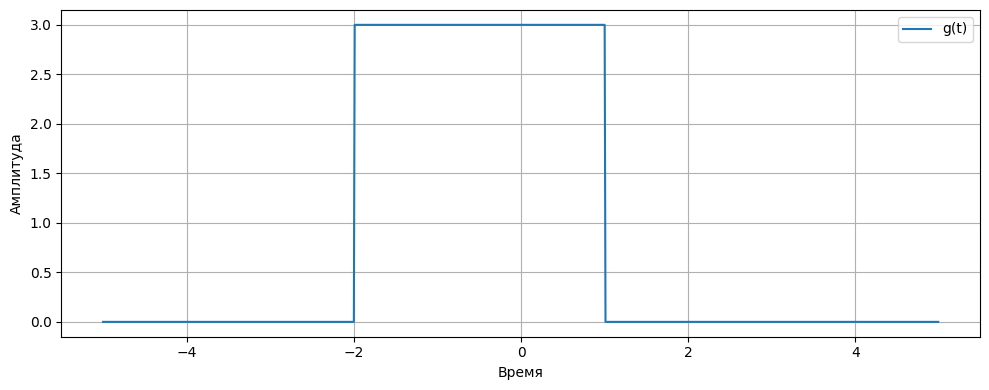
\includegraphics[width=0.8\textwidth]{src/signal.png}
    \caption{График функции \(g(t)\)}              
\end{figure}
\noindent
Также нужно задать зашумлённую версию нашего сигнала, которая имеет вид:
\[
u(t)=g(t)+b\,\xi(t)+c\sin{dt},
\]
где \(\xi(t)\) – белый шум (равномерно распределённый на \([-1,1]\)), а \(b, c, d\) --- параметры возмущения.

\addsubsection{Убираем высокие частоты}
При выполнении этого пункта гармоническая составляющая отсутствует (\(c=0\)). Таким образом к исходному сигналу добавляется только белый шум с коэффициентом $b$. Сигнал принимает вид:
\[u(t) = g(t) + b \cdot \xi(t),\]
где $\xi(t)$ --- белый шум, равномерно распределённый на интервале $[-1,1]$. Параметр $b$ зададим как множество значений $b = \{0.1, 1.0, 3.0\}$. Для каждого значения $b$ построим графики временных сигналов и спектров:
\begin{figure}[H]
    \centering
    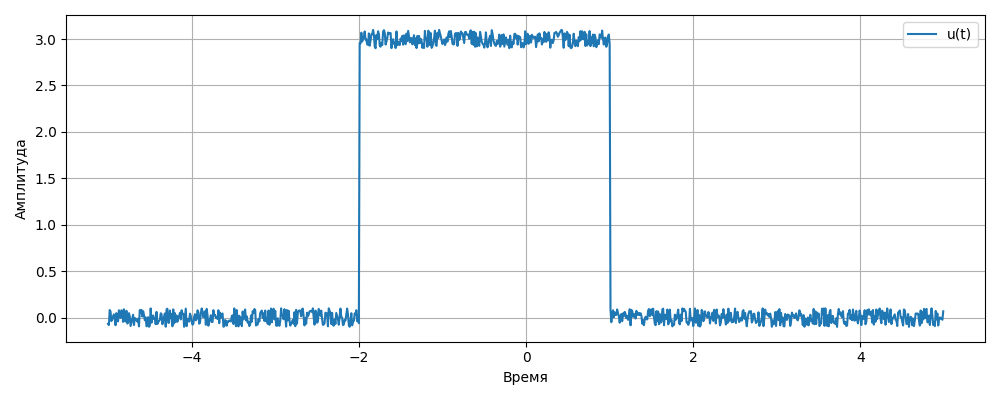
\includegraphics[width=0.8\textwidth]{src/time_0.1.png}
    \caption{График зашумленного сигнала при $b=0.1$}
\end{figure}
\begin{figure}[H]
    \centering
    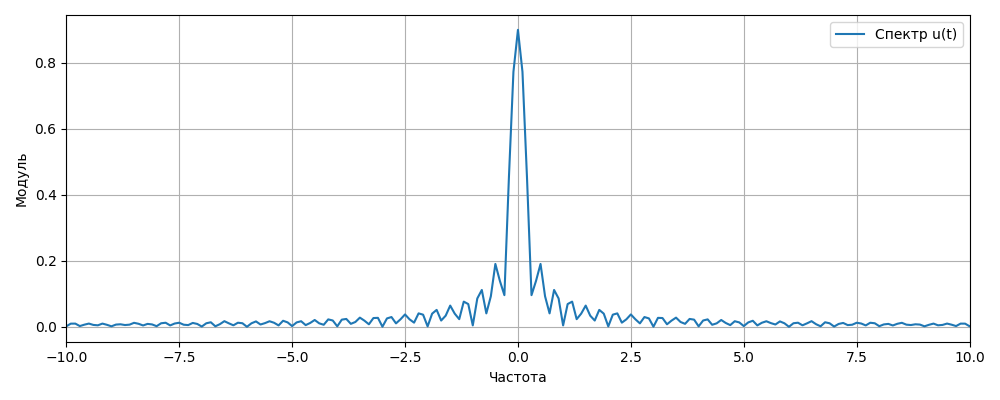
\includegraphics[width=0.8\textwidth]{src/spec_0.1.png}
    \caption{График Фурье-образа сигнала при $b=0.1$}
\end{figure}
\begin{figure}[H]
    \centering
    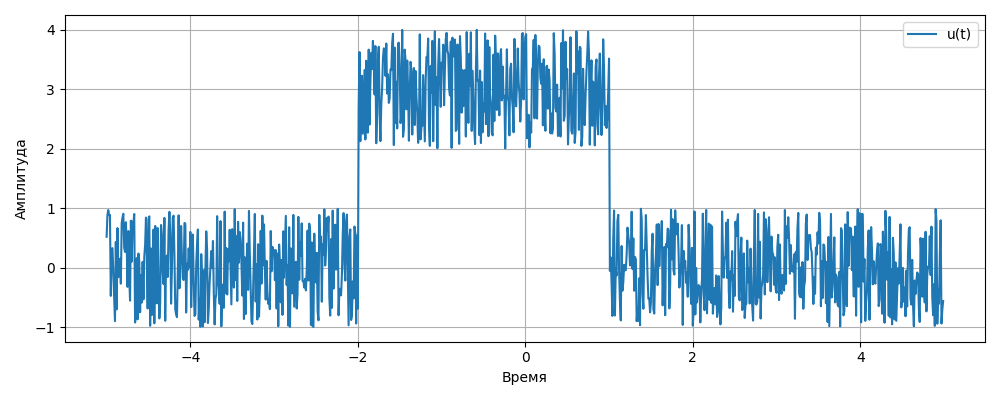
\includegraphics[width=0.8\textwidth]{src/time_1.0.png}
    \caption{График зашумленного сигнала при $b=1.0$}
\end{figure}
\begin{figure}[H]
    \centering
    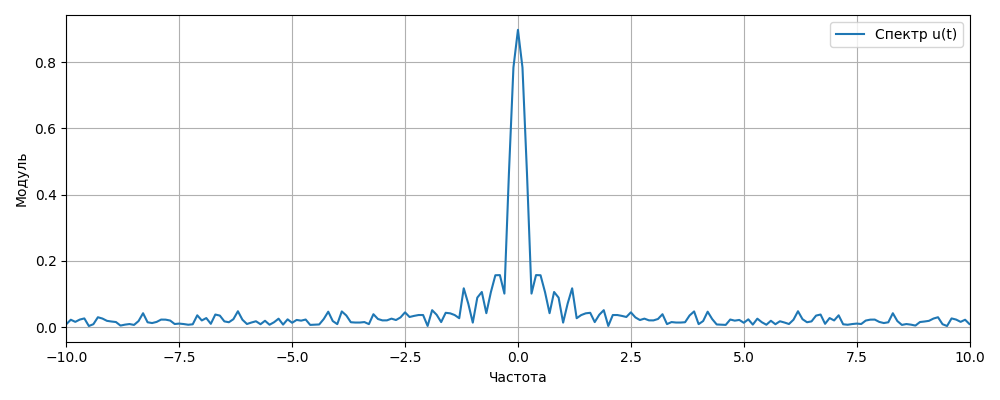
\includegraphics[width=0.8\textwidth]{src/spec_1.0.png}
    \caption{График Фурье-образа сигнала при $b=1.0$}
\end{figure}
\begin{figure}[H]
    \centering
    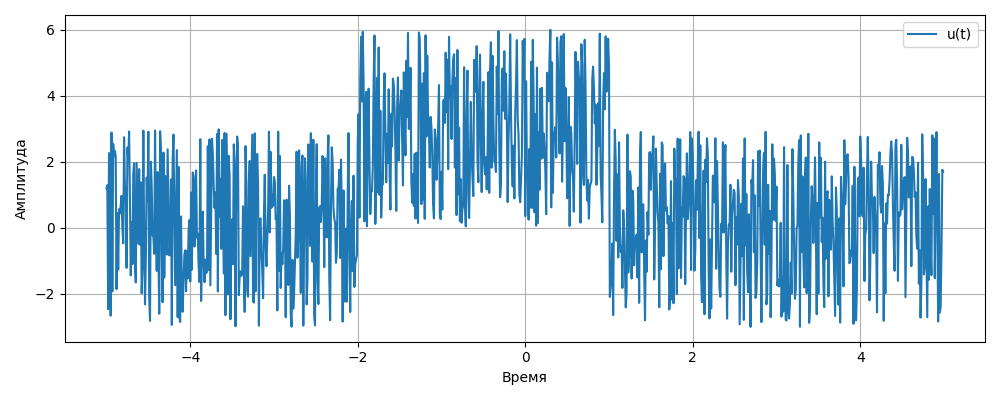
\includegraphics[width=0.8\textwidth]{src/time_3.0.png}
    \caption{График зашумленного сигнала при $b=3.0$}
\end{figure}
\begin{figure}[H]
    \centering
    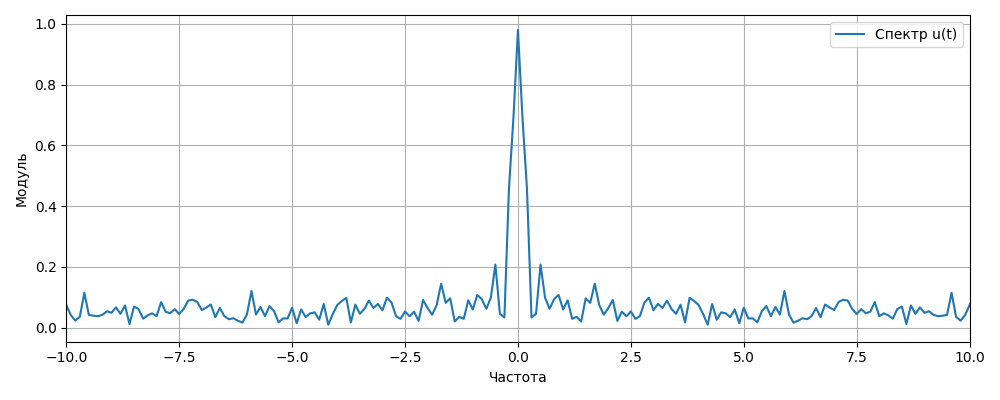
\includegraphics[width=0.8\textwidth]{src/spec_3.0.png}
    \caption{График Фурье-образа сигнала при $b=3.0$}
\end{figure}
\noindent
Исходя из графиков можем сделать вывод, что при увеличении параметра $b$ увеличивается уровень шума в сигнале, что приводит к более выраженному рассеянию спектральных компонент.

Теперь посмотрим на то, как параметры $b$ и $\nu_0$ влияют на эффективность фильтрации. К каждому значению параметра $b$ будем перебирать значения параметра $\nu_0$, который зададим как множество значений $\nu_0 = \{1.0, 5.0, 10.0\}$. Для каждой пары значений построим 2 сравнительных графика. Первый включает в себя графики исходного сигнала, его зашумленную версию и версию с применением фильтра низких частот. Второй будет включать модули Фурье-образов для каждого из сигналов.\\ [0.5em]
Пусть параметр $b=0.1$, переберем значения параметра $\nu_0$:
\begin{figure}[H]
    \centering
    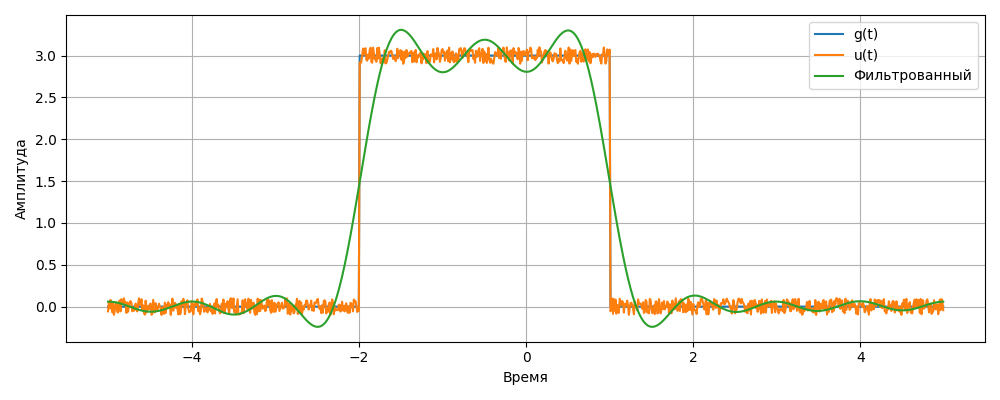
\includegraphics[width=0.8\textwidth]{src/lpf/time_0.1_1.0.png}
    \caption{Сравнительные временные графики при $b=0.1$ и $\nu_0=1.0$}
\end{figure}
\begin{figure}[H]
    \centering
    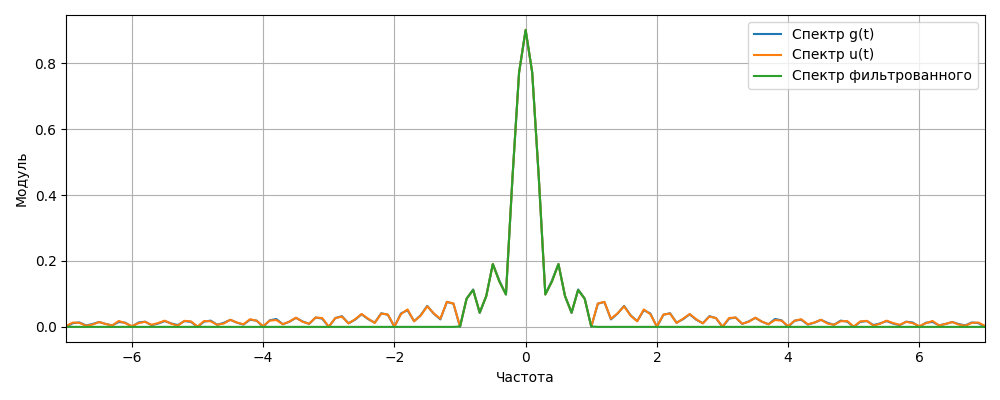
\includegraphics[width=0.8\textwidth]{src/lpf/spec_0.1_1.0.png}
    \caption{Сравнительные спектры при $b=0.1$ и $\nu_0=1.0$}
\end{figure}
\begin{figure}[H]
    \centering
    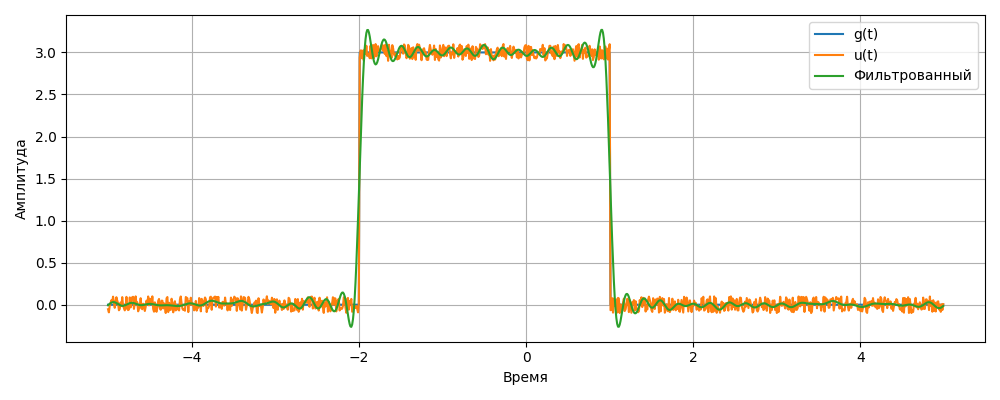
\includegraphics[width=0.8\textwidth]{src/lpf/time_0.1_5.0.png}
    \caption{Сравнительные временные графики при $b=0.1$ и $\nu_0=5.0$}
\end{figure}
\begin{figure}[H]
    \centering
    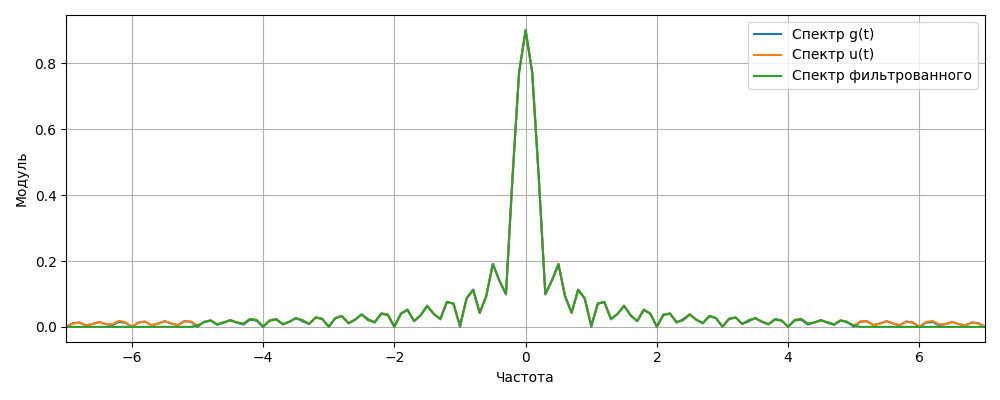
\includegraphics[width=0.8\textwidth]{src/lpf/spec_0.1_5.0.png}
    \caption{Сравнительные спектры при $b=0.1$ и $\nu_0=5.0$}
\end{figure}
\begin{figure}[H]
    \centering
    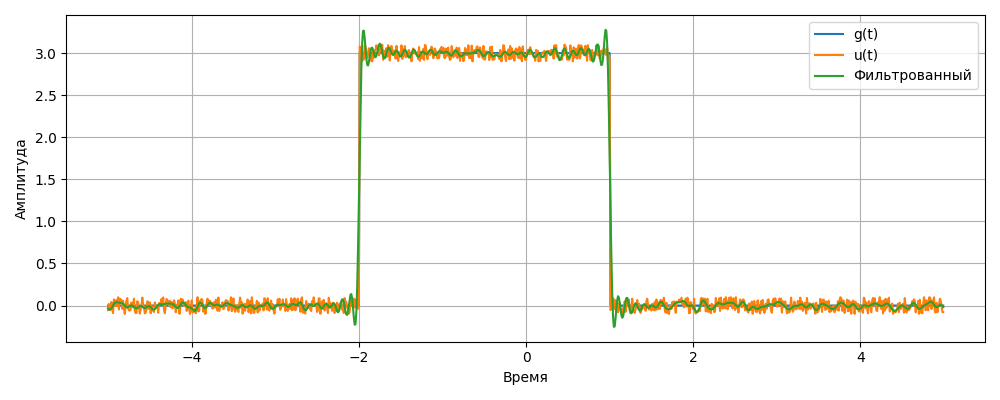
\includegraphics[width=0.8\textwidth]{src/lpf/time_0.1_10.0.png}
    \caption{Сравнительные временные графики при $b=0.1$ и $\nu_0=10.0$}
\end{figure}
\begin{figure}[H]
    \centering
    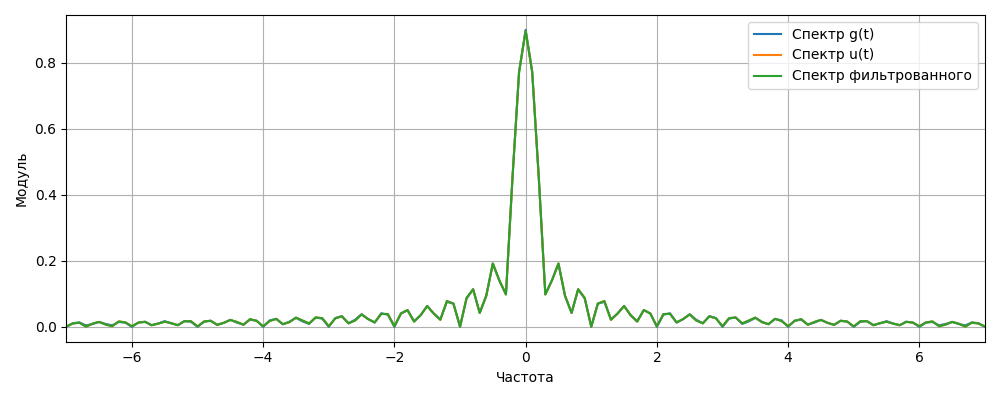
\includegraphics[width=0.8\textwidth]{src/lpf/spec_0.1_10.0.png}
    \caption{Сравнительные спектры при $b=0.1$ и $\nu_0=10.0$}
\end{figure}
\noindent
Мы видим, что при $\nu_0=1$  спектре остаются только самые низкие частоты, поэтому резкие фронты исходного прямоугольного сигнала сглаживаются. На временном графике видно, что фильтрованный сигнал повторяет общую форму $g(t)$, но переходы становятся более пологими, что говорит о потере высокочастотных составляющих, важных для чёткого воспроизведения прямоугольных границ. \\ [0.5em]
При $\nu_0=5$ баланс между сохранением формы сигнала и удалением шума становится лучше. Фильтрованный сигнал в целом ближе к исходному $g(t)$, а шумовая составляющая заметно подавлена. \\ [0.5em]
При $\nu_0=10$ пропускается более широкий диапазон частот, что позволяет лучше восстановить резкие переходы прямоугольника. Однако при этом часть высокочастотного шума также сохраняется.

Таким образом, при невысоком уровне шума оптимальным с точки зрения компромисса между удалением шума и сохранением резких границ может считаться промежуточное значение частоты среза, то есть $\nu_0=5$.

Теперь $b=1.0$, снова переберем значения параметра $\nu_0$:
\begin{figure}[H]
    \centering
    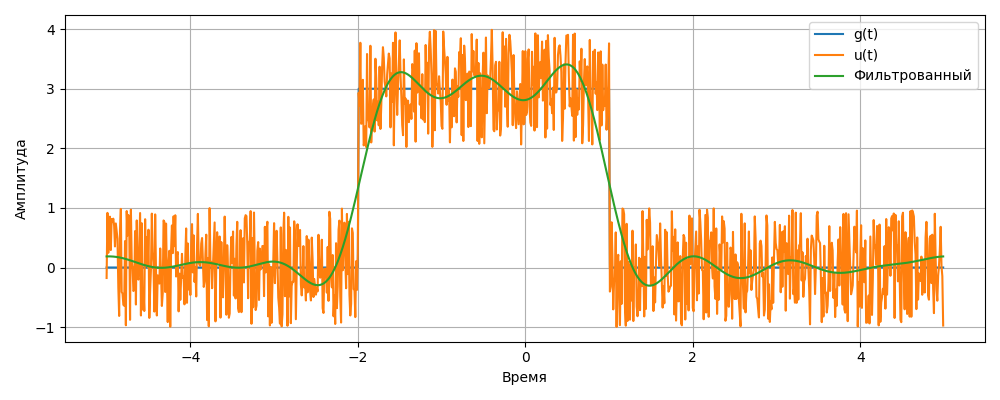
\includegraphics[width=0.8\textwidth]{src/lpf/time_1.0_1.0.png}
    \caption{Сравнительные временные графики при $b=1.0$ и $\nu_0=1.0$}
\end{figure}
\begin{figure}[H]
    \centering
    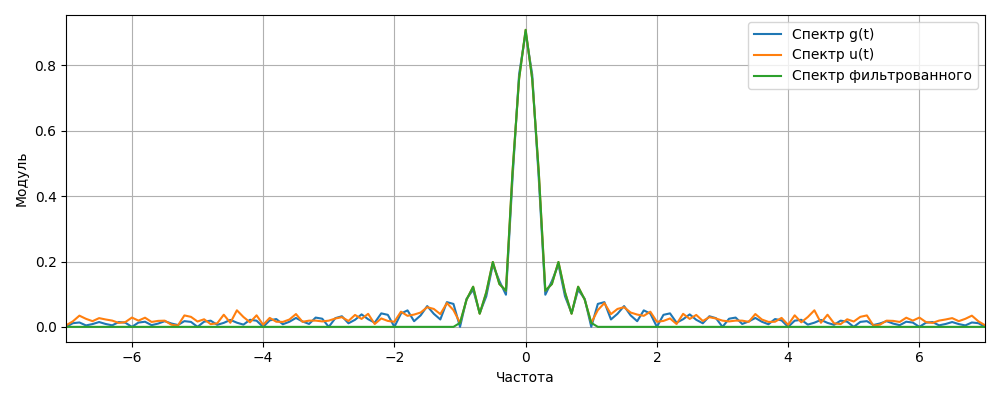
\includegraphics[width=0.8\textwidth]{src/lpf/spec_1.0_1.0.png}
    \caption{Сравнительные спектры при $b=1.0$ и $\nu_0=1.0$}
\end{figure}
\begin{figure}[H]
    \centering
    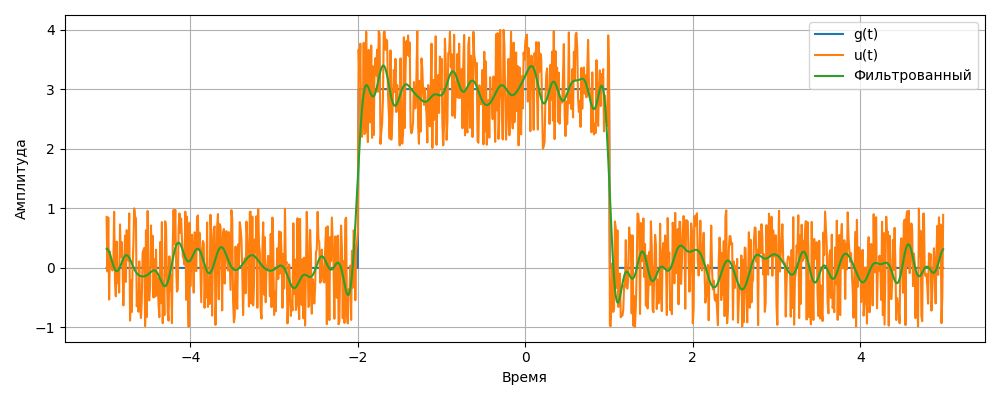
\includegraphics[width=0.8\textwidth]{src/lpf/time_1.0_5.0.png}
    \caption{Сравнительные временные графики при $b=1.0$ и $\nu_0=5.0$}
\end{figure}
\begin{figure}[H]
    \centering
    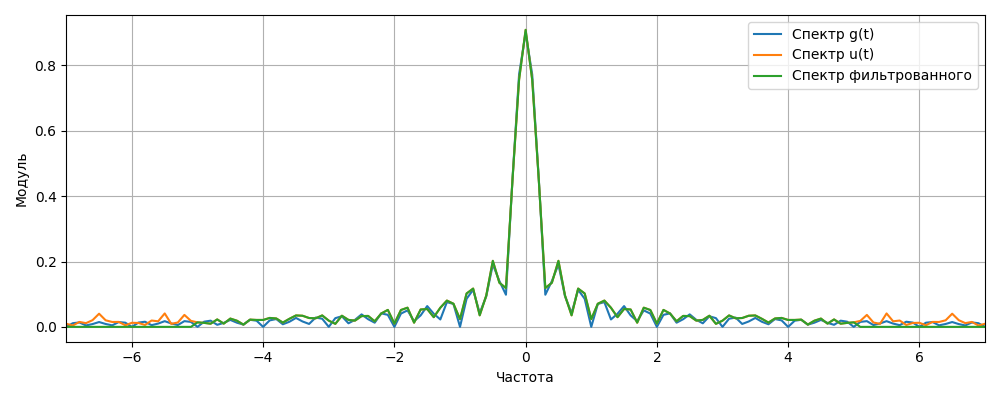
\includegraphics[width=0.8\textwidth]{src/lpf/spec_1.0_5.0.png}
    \caption{Сравнительные спектры при $b=1.0$ и $\nu_0=5.0$}
\end{figure}
\begin{figure}[H]
    \centering
    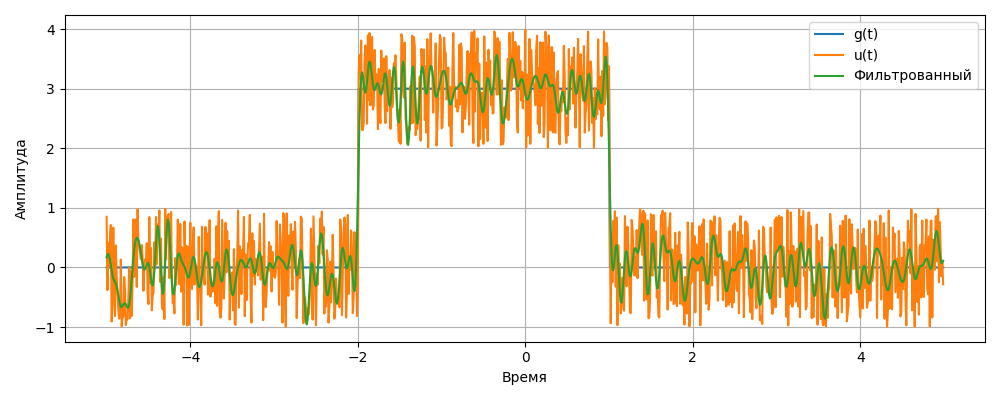
\includegraphics[width=0.8\textwidth]{src/lpf/time_1.0_10.0.png}
    \caption{Сравнительные временные графики при $b=1.0$ и $\nu_0=10.0$}
\end{figure}
\begin{figure}[H]
    \centering
    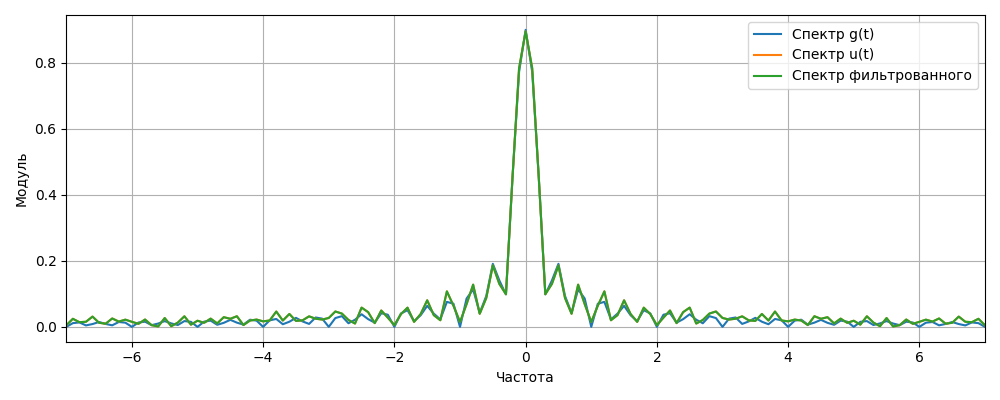
\includegraphics[width=0.8\textwidth]{src/lpf/spec_1.0_10.0.png}
    \caption{Сравнительные спектры при $b=1.0$ и $\nu_0=10.0$}
\end{figure}
\noindent
Проанализировав графики делаем вывод, что при повышенном уровне шума слишком низкая частота среза $\nu_0$ чрезмерно сглаживает сигнал, а слишком высокая --- пропускает заметную часть шума. И снова оптимальным значением можно считать $\nu_0 = 5.0$.

Посмотрим на случай $b=3.0$:
\begin{figure}[H]
    \centering
    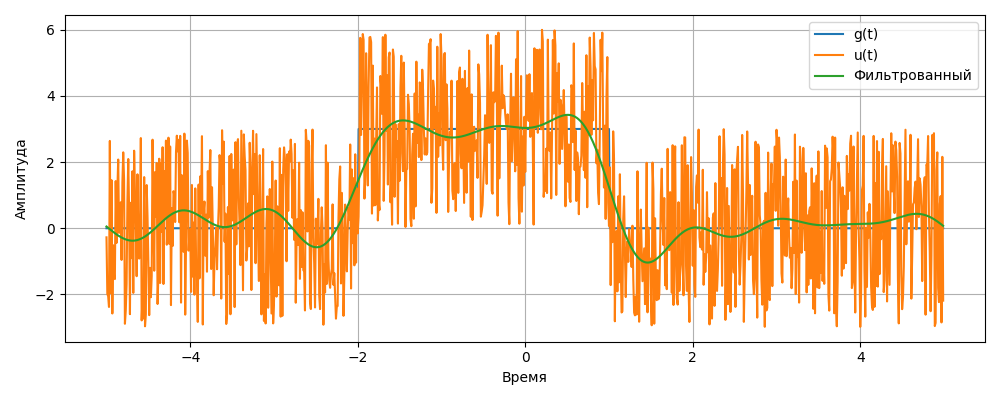
\includegraphics[width=0.8\textwidth]{src/lpf/time_3.0_1.0.png}
    \caption{Сравнительные временные графики при $b=3.0$ и $\nu_0=1.0$}
\end{figure}
\begin{figure}[H]
    \centering
    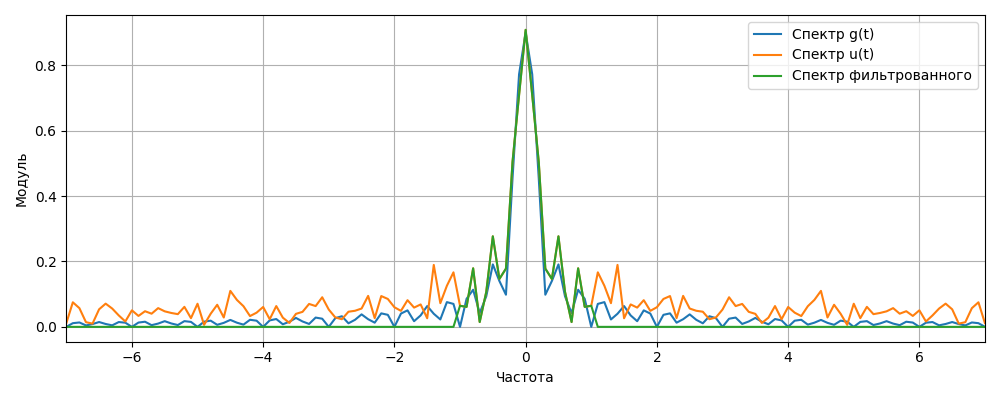
\includegraphics[width=0.8\textwidth]{src/lpf/spec_3.0_1.0.png}
    \caption{Сравнительные спектры при $b=3.0$ и $\nu_0=1.0$}
\end{figure}
\begin{figure}[H]
    \centering
    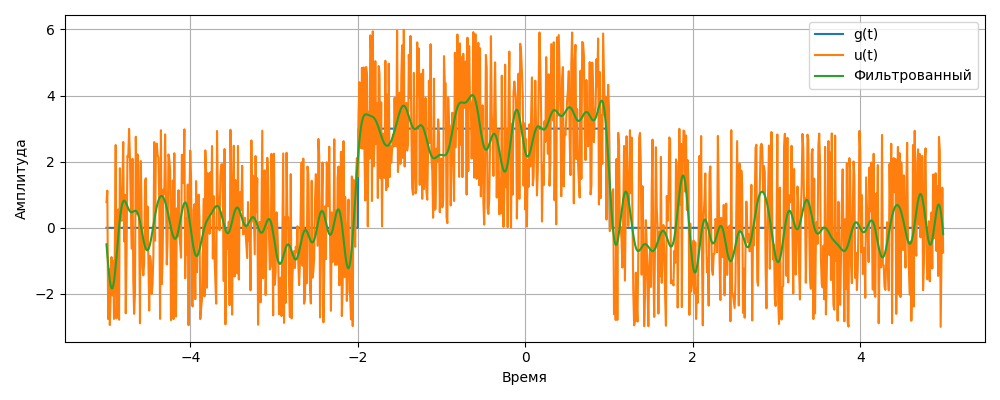
\includegraphics[width=0.8\textwidth]{src/lpf/time_3.0_5.0.png}
    \caption{Сравнительные временные графики при $b=3.0$ и $\nu_0=5.0$}
\end{figure}
\begin{figure}[H]
    \centering
    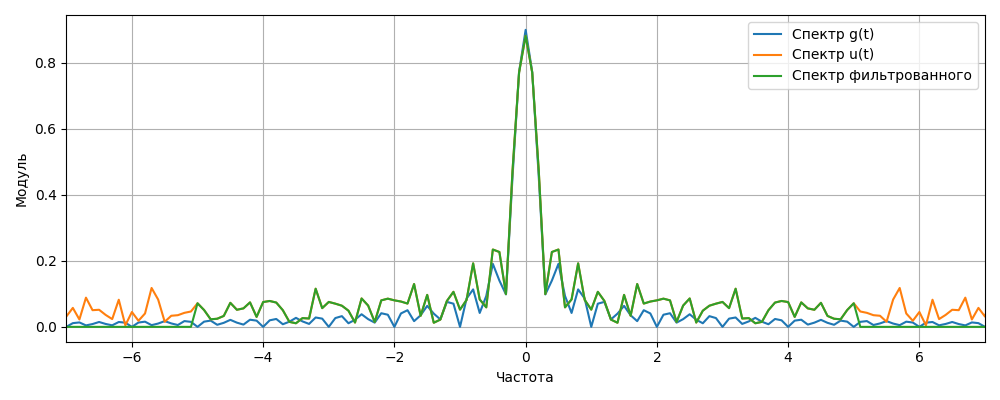
\includegraphics[width=0.8\textwidth]{src/lpf/spec_3.0_5.0.png}
    \caption{Сравнительные спектры при $b=3.0$ и $\nu_0=5.0$}
\end{figure}
\begin{figure}[H]
    \centering
    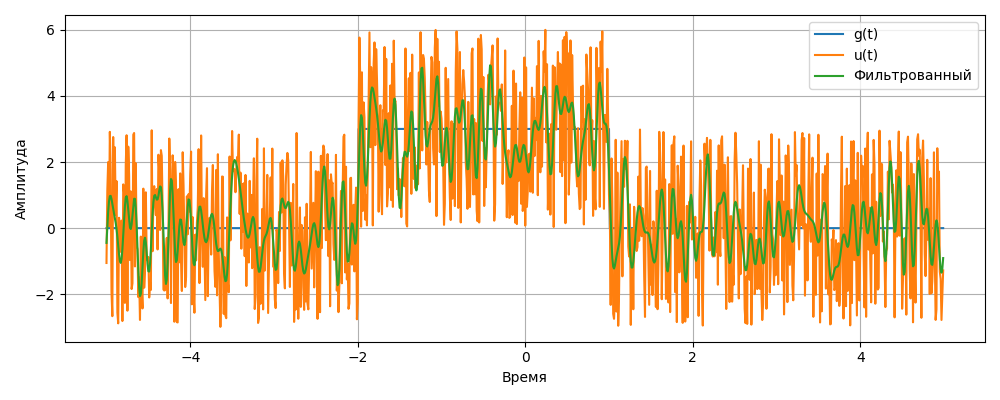
\includegraphics[width=0.8\textwidth]{src/lpf/time_3.0_10.0.png}
    \caption{Сравнительные временные графики при $b=3.0$ и $\nu_0=10.0$}
\end{figure}
\begin{figure}[H]
    \centering
    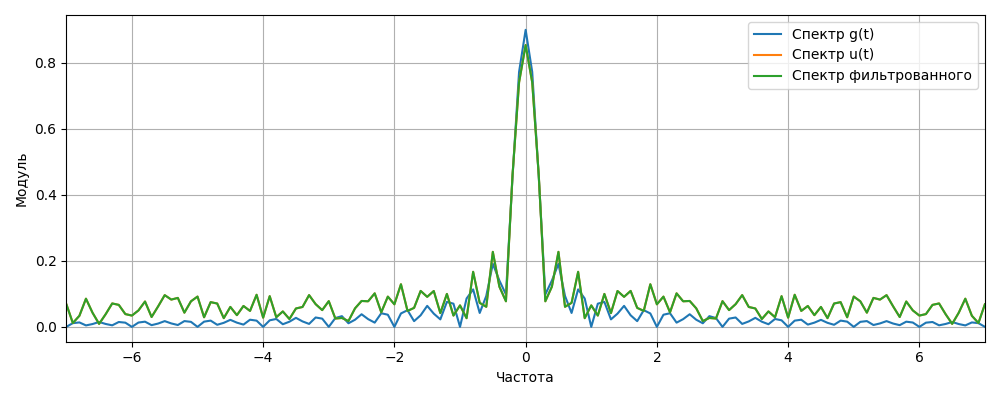
\includegraphics[width=0.8\textwidth]{src/lpf/spec_3.0_10.0.png}
    \caption{Сравнительные спектры при $b=3.0$ и $\nu_0=10.0$}
\end{figure}
\noindent           
Анализ совокупности полученных графиков при различных значениях коэффициента шума $b$ и частоты среза $\nu_0$ показывает следующее:
\begin{itemize}
    \item При слишком низкой частоте среза ($\nu_0=1$) хорошо подавляются шумовые компоненты, но резкие переходы исходного прямоугольного сигнала сглаживаются.
    \item При слишком высокой частоте среза ($\nu_0=10$) сохраняются фронты сигнала, однако шумовая составляющая остаётся заметной.
    \item Оптимальным компромиссом между подавлением шума и сохранением формы сигнала оказалась промежуточная частота среза ($\nu_0=5$). 
    \item Для значений $b \approx 0.1\text{--}1.0$ фильтр при $\nu_0=5$ восстанавливает форму прямоугольника достаточно хорошо и при этом существенно подавляет шум.
\end{itemize}
Таким образом, при решении задачи жёсткой фильтрации нижних частот для заданных параметров сигнала наилучшие результаты даёт частота среза $\nu_0 \approx 5$ при умеренном уровне шума ($b \approx 0.1\text{--}1.0$).

\addsubsection{Убираем специфические частоты}
В этом пункте рассмотрим случай, когда в сигнале присутствуют оба вида помех:
\begin{itemize}
    \item Белый шум с коэффициентом $b \neq 0$,
    \item Гармоническая составляющая $c \sin(d \, t)$.
\end{itemize}
Тогда зашумлённый сигнал примет вид:
\[
    u(t) = g(t) + b \cdot \xi(t) + c \sin(d \, t),
\]
где $\xi(t)$ --- белый шум, равномерно распределённый на интервале $[-1,1]$. \\[0.5em]
Для устранения одновременно и белого шума, и гармонической помехи воспользуемся совмещённым жёстким фильтром, который состоит из:
\begin{enumerate}
    \item Фильтра нижних частот с частотой среза $\nu_0$ который мы рассмотрели ранее.
    \item Notch-фильтра, который обнуляет спектр в узкой полосе вокруг частоты $\pm \frac{d}{2\pi}$. Тем самым удаляется гармоника $\sin(d \, t)$.
\end{enumerate}
Давайте зададим необходимые параметры и приступим к анализу. Пусть $b \in \{\,0.0,\,1.0,\,2.0\}$, $c \in \{\,0.5,\,1.0\}$, $d \in \{\,5.0,\,10.0\}$, $\nu_0 \in \{\,4.0,\,8.0\}$. Ширину выреза вокруг $d$ возьмём $\delta = 0.3$. 

Далее в отчете я приведу лишь те графики, которые наиболее наглядно иллюстрируют влияние параметров на результат фильтрации. Остальные графики можно найти в \href{https://drive.google.com/drive/folders/1fi6P5S0JTVP9--mFtsujHoE6mchsh4uM?usp=sharing}{облаке}.
\begin{figure}[H]
    \centering
    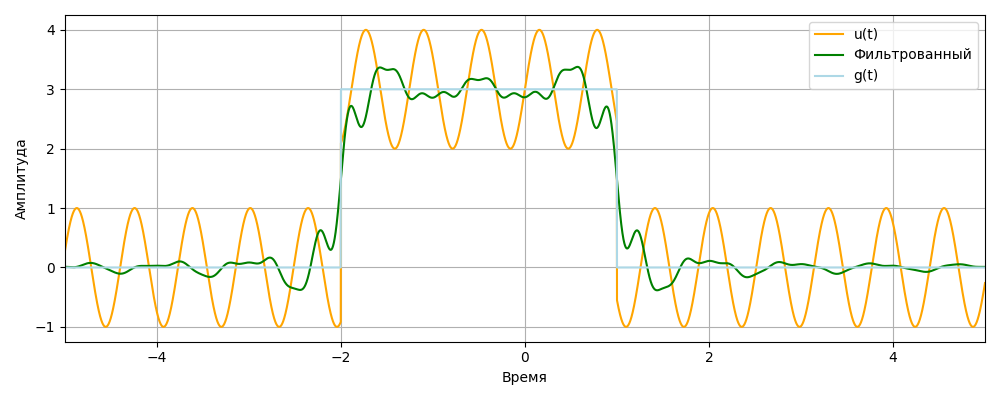
\includegraphics[width=0.8\textwidth]{src/npf/time_0_1.0_10.0_4.0.png}
    \caption{Сравнительные временные графики при $b=0.0$, $c=1.0$, $d=10.0$, $\nu_0=4.0$}
\end{figure}
\begin{figure}[H]
    \centering
    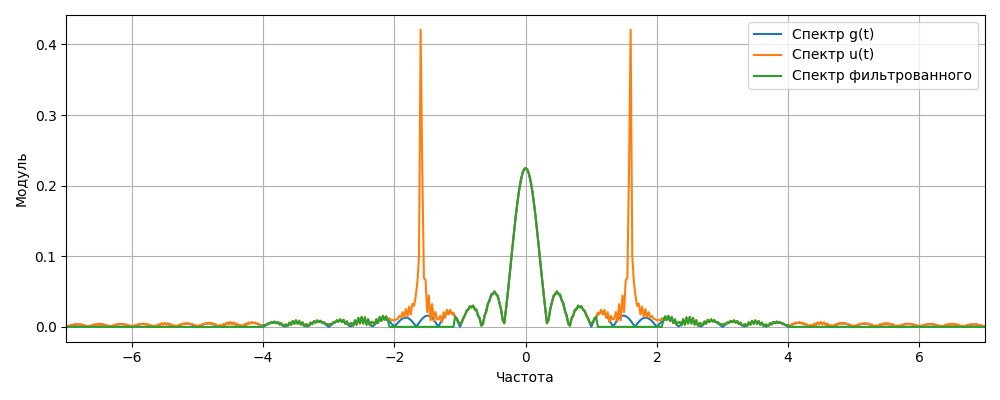
\includegraphics[width=0.8\textwidth]{src/npf/spec_0_1.0_10.0_4.0.png}
    \caption{Сравнительные спектры при $b=0.0$, $c=1.0$, $d=10.0$, $\nu_0=4.0$}
\end{figure}
На графиках показан случай, когда в сигнале отсутствует белый шум ($b=0$), но присутствует гармоническая помеха с параметрами $c=1.0$ и $d=10.0$. Применяем совмещённый фильтр (низкочастотный с $\nu_0=4.0$ и Notch вокруг $\pm \frac{d}{2\pi}$). Видно, что:
\begin{itemize}
    \item Временной сигнал после фильтрации (зелёная кривая) заметно стремится к исходнному прямоугольнику (голубая кривая), поскольку шум отсутствует и надо было лишь убрать гармонику.
    \item На спектре исчезают выраженные пики на частотах $\pm \frac{d}{2\pi}$, соответствующие гармонике $c\,\sin(d\,t)$. При этом сохраняется центральная часть спектра, отвечающая форме прямоугольного сигнала.
\end{itemize}

\begin{figure}[H]
    \centering
    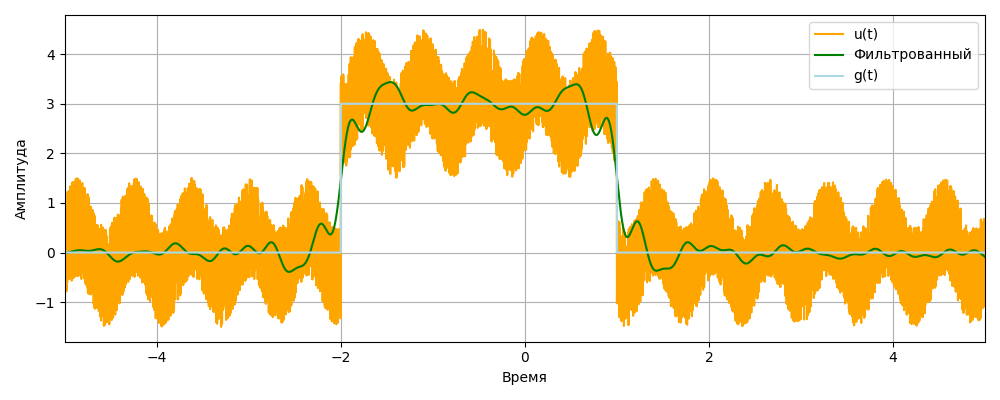
\includegraphics[width=0.8\textwidth]{src/npf/time_1.0_0.5_10.0_4.0.png}
    \caption{Сравнительные временные графики при $b=1.0$, $c=0.5$, $d=10.0$, $\nu_0=4.0$}
\end{figure}
\begin{figure}[H]
    \centering
    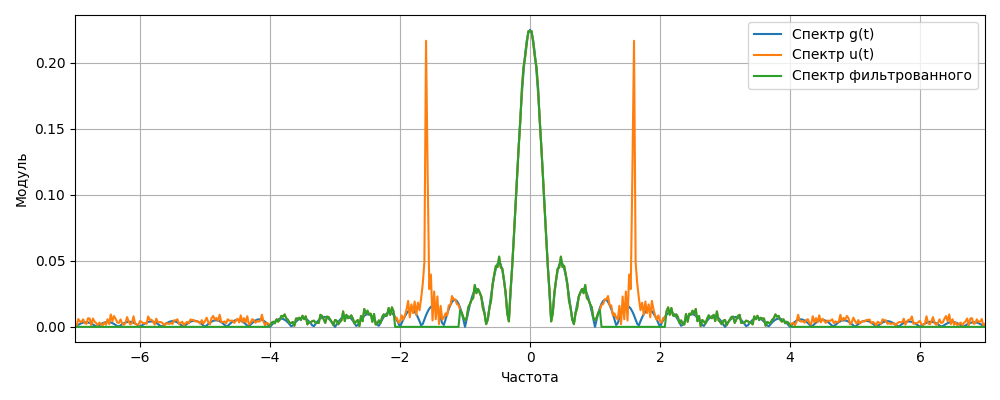
\includegraphics[width=0.8\textwidth]{src/npf/spec_1.0_0.5_10.0_4.0.png}
    \caption{Сравнительные спектры при $b=1.0$, $c=0.5$, $d=10.0$, $\nu_0=4.0$}
\end{figure}
На этих графиках изображён сигнал при умеренном уровне белого шума $b=1.0$ и меньшей амплитуде гармоники $c=0.5$ (частота $d=10.0$, $\nu_0=4.0$). Здесь:
\begin{itemize}
    \item Оранжевая область на временном графике показывает диапазон шума: видим, что при $b=1.0$ <<толщина>> шумовой полосы не слишком велика, и фильтр (зелёная кривая) в целом восстанавливает прямоугольник.
    \item На спектре основной пик гармоники при $\pm \frac{d}{2\pi}$ меньше, чем в предыдущем случае ($c=0.5$ вместо $c=1.0$), но всё равно отчётливо подавляется Notch-фильтром. Высокочастотные шумовые компоненты также частично срезаны.
\end{itemize}

\begin{figure}[H]
    \centering
    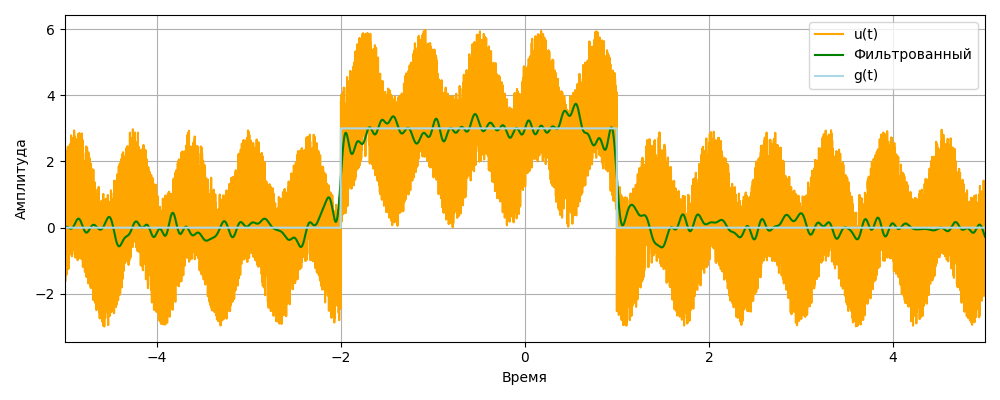
\includegraphics[width=0.8\textwidth]{src/npf/time_2.0_1.0_10.0_8.0.png}
    \caption{Сравнительные временные графики при $b=2.0$, $c=1.0$, $d=10.0$, $\nu_0=8.0$}
\end{figure}
\begin{figure}[H]
    \centering
    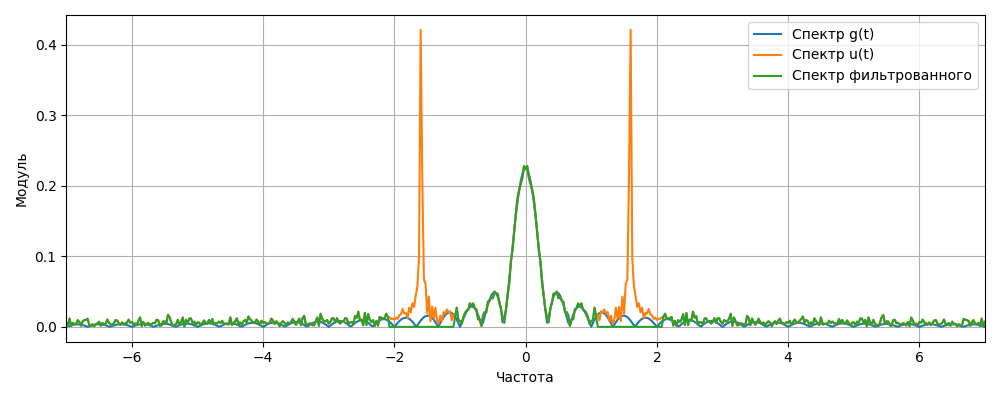
\includegraphics[width=0.8\textwidth]{src/npf/spec_2.0_1.0_10.0_8.0.png}
    \caption{Сравнительные спектры при $b=2.0$, $c=1.0$, $d=10.0$, $\nu_0=8.0$}
\end{figure}

Далее, мы видим пример более сильного шума ($b=2.0$) и более широкого диапазона пропускания ($\nu_0=8.0$), при этом $c=1.0$ и $d=10.0$. Сравнивая с предыдущими случаями, видим:
\begin{itemize}
    \item Шумовая <<полоса>> (оранжевый цвет) стала шире, так как $b=2.0$ заметно повышает амплитуду белого шума.
    \item Повышенная частота среза $\nu_0=8.0$ лучше сохраняет резкие переходы прямоугольника, но при этом часть шума просачивается в итоговый сигнал (зелёная кривая). 
\end{itemize}
\noindent Таким образом, из рассмотренных графиков можно сделать несколько ключевых наблюдений:
\begin{itemize}
    \item При отсутствии белого шума ($b=0$) достаточно убрать гармоническую помеху с помощью Notch-фильтра; выбор $\nu_0$ лишь влияет на сохранение резких переходов прямоугольника.
    \item При умеренном шуме (например, $b=1.0$) фильтр низких частот помогает убрать шумовые компоненты, а Notch-фильтр --- гармонику. Компромиссное значение $\nu_0$ (около 4--5) часто даёт хорошее сочетание подавления шума и сохранения формы сигнала.
    \item При большом $b=2.0$ (сильном шуме) для сохранения фронтов желательно повышать $\nu_0$, но тогда часть шума попадает в итоговый сигнал. Следовательно, выбирается баланс между сохранением резких переходов и подавлением шума.
    \item Во всех случаях Notch-фильтр эффективно устраняет гармонику с частотой $d$, причём важно корректно задать ширину полосы выреза, чтобы полностью подавить пик на $\pm \frac{d}{2\pi}$, не затронув избыточно соседние частоты прямоугольного импульса.
\end{itemize}

\addsubsection{Убираем низкие частоты}
В третьем пункте рассмотрим фильтр, который обнуляет все спектральные компоненты в некоторой окрестности нулевой частоты, то есть при $|f| < \nu_0$. Другими словами, это фильтр высоких частот (High-Pass Filter), который вырезает низкочастотную часть сигнала. \\[0.5em]
Для наглядности зададим пару значений параметра $\nu_0 = [4.0, 8.0]$ и посмотрим, как влияет такой <<срез>> на прямоугольный сигнал $g(t)$, к которому добавлены белый шум и гармоническая составляющая. Пусть зашумлённая версия имеет вид как в прошлом задании. \\[0.5em] 
Построим графики и посмотрим на результаты.
\begin{figure}[H]
    \centering
    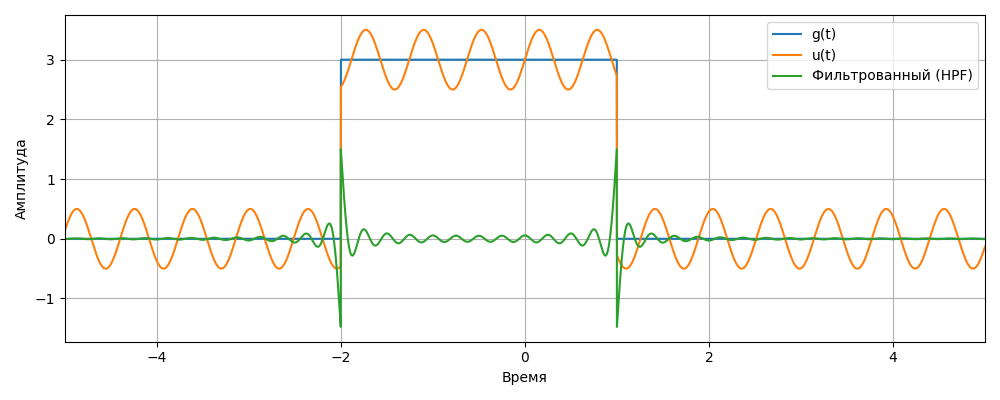
\includegraphics[width=0.8\textwidth]{src/hpf/time_0_0.5_10.0_4.0.png}
    \caption{Сравнительные временные сигналы при $b=0.0$, $c=0.5$, $d=10.0$, $\nu_0=4.0$}
\end{figure}
\begin{figure}[H]
    \centering
    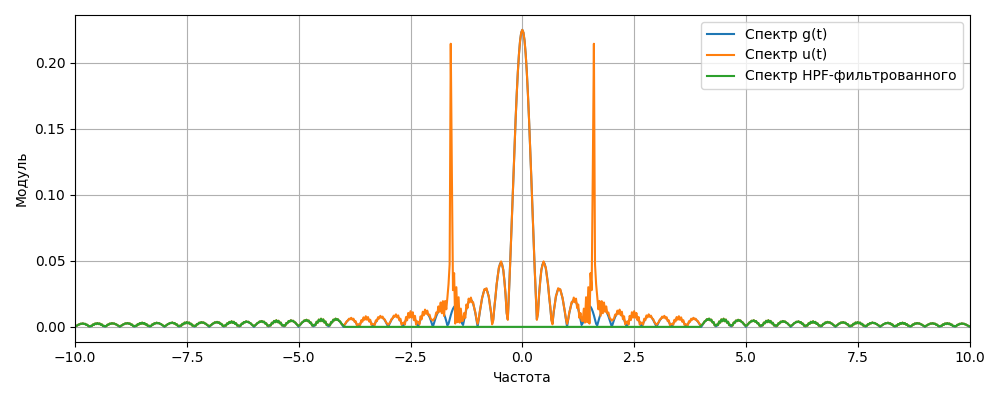
\includegraphics[width=0.8\textwidth]{src/hpf/spec_0_0.5_10.0_4.0.png}
    \caption{Сравнительные спектры при $b=0.0$, $c=0.5$, $d=10.0$, $\nu_0=4.0$}
\end{figure}
Здесь мы видим, что:
\begin{itemize}
    \item Временной сигнал после фильтрации сохраняет высокочастотные колебания, однако теряет <<ступенчатую>> структуру исходного прямоугольника. 
    \item На спектральном графике отчётливо видно обнуление области $|f| < 2.0$, что приводит к исчезновению медленных переходов и постоянной составляющей.
\end{itemize}

Теперь стоит рассмотреть случай более сильного шума ($b=2.0$) и более высокого значения $\nu_0=8.0$. 
\begin{figure}[H]
    \centering
    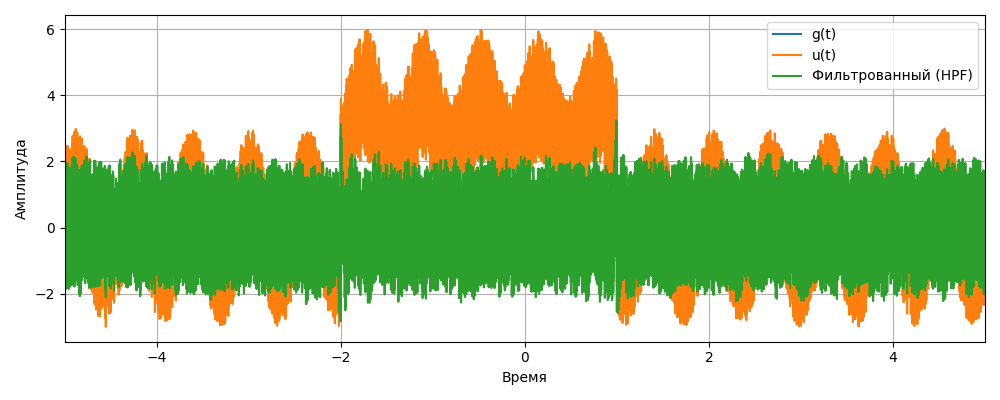
\includegraphics[width=0.8\textwidth]{src/hpf/time_2.0_1.0_10.0_8.0.png}
    \caption{Сравнительные временные сигналы при $b=2.0$, $c=1.0$, $d=10.0$, $\nu_0=8.0$}
\end{figure}
\begin{figure}[H]
    \centering
    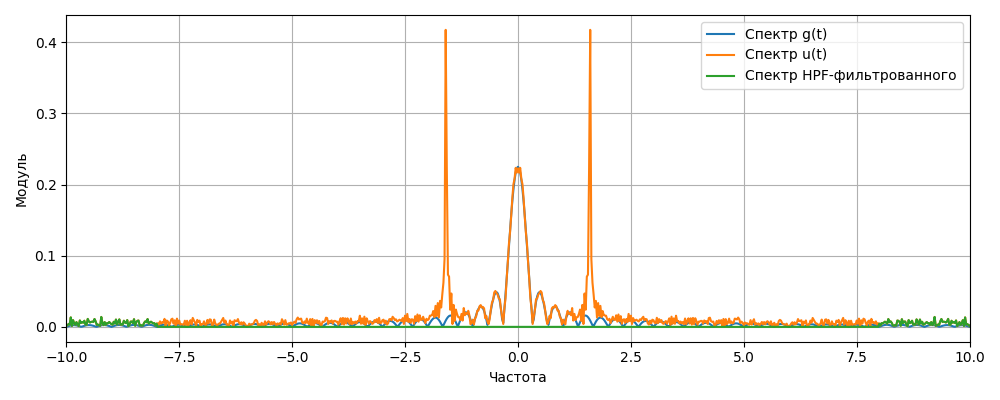
\includegraphics[width=0.8\textwidth]{src/hpf/spec_2.0_1.0_10.0_8.0.png}
    \caption{Сравнительные спектры при $b=2.0$, $c=1.0$, $d=10.0$, $\nu_0=8.0$}
\end{figure}
На графиках видно, что:
\begin{itemize}
    \item Фронты прямоугольника становятся ещё менее выраженными, так как низкочастотная часть сигнала полностью <<вырезана>>.
    \item Высокочастотный шум проходит через фильтр, делая итоговый сигнал заметно <<колеблющимся>>.
\end{itemize}

Таким образом, фильтр, который вырезает низкие частоты, может быть полезен для удаления медленных трендов или постоянной компоненты, но не подходит для восстановления прямоугольных сигналов с резкими переходами.

\addsection{Задание 2. Фильтрация звука}
В этом задании требуется выделить голос из аудиозаписи, в которой присутствуют посторонние шумы. В качестве входных данных используем файл \texttt{MUHA.wav}, содержащий речевой фрагмент с различными помехами. Необходимо отфильтровать исходный сигнал, чтобы максимально подавить шум и оставить только человеческий голос.

Для этого с помощью функций чтения аудиофайла получаем массив отсчётов сигнала и частоту дискретизации.\\[0.5em] 
Посмотрим на график временного сигнала и спектрограмму записи, чтобы оценить, какие частоты преобладают в аудиофайле и какие шумы присутствуют.
\begin{figure}[H]
    \centering
    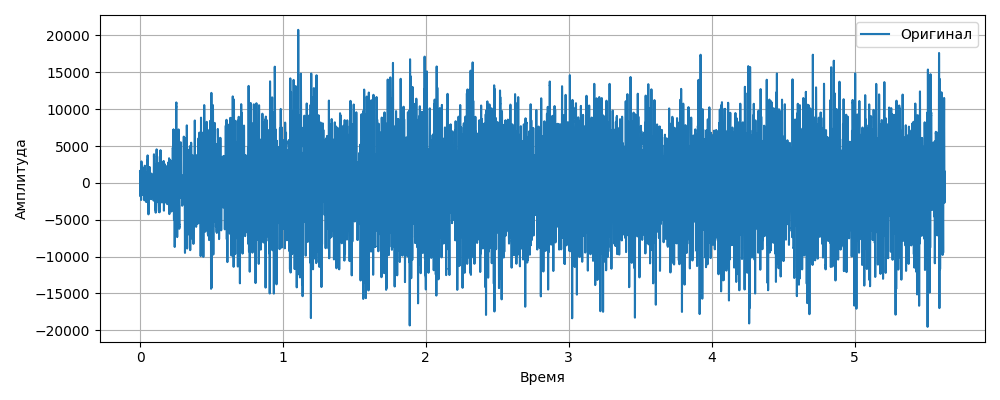
\includegraphics[width=0.8\textwidth]{src/time_orig_rec.png}
    \caption{Временной сигнал исходной записи}
\end{figure}

\begin{figure}[H]
    \centering
    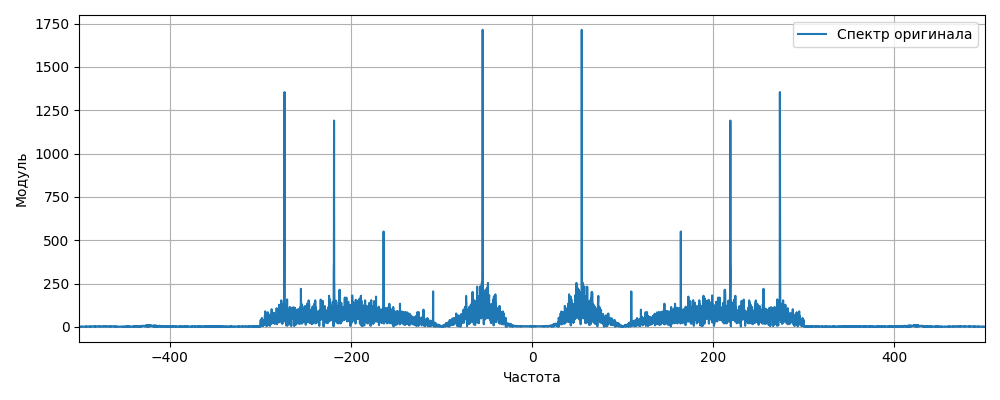
\includegraphics[width=0.8\textwidth]{src/spec_orig_rec.png}
    \caption{Спектр сигнала исходной записи}
\end{figure}

Можно обратить внимание, что шум присутсвует в диапазоне частот от $0$ до $\sim 300$ Гц. Для простоты фильтрации будем использовать полосовой жёсткий фильтр, который оставит только частоты в определенном диапазоне. \\[0.5em]
Применим его и построим графики для сравнения исходного и отфильтрованного сигналов.
\begin{figure}[H]
    \centering
    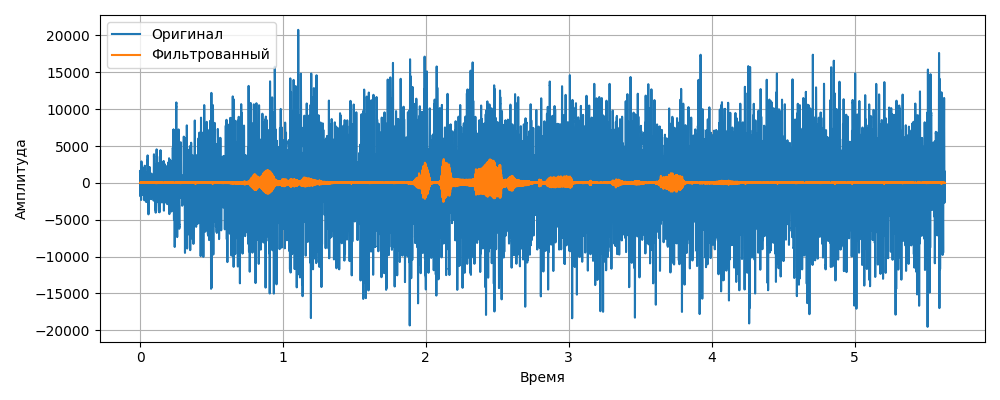
\includegraphics[width=0.8\textwidth]{src/time_orig_filter_rec.png}
    \caption{Временные сигналы: исходный и фильтрованный}
\end{figure}
\begin{figure}[H]
    \centering
    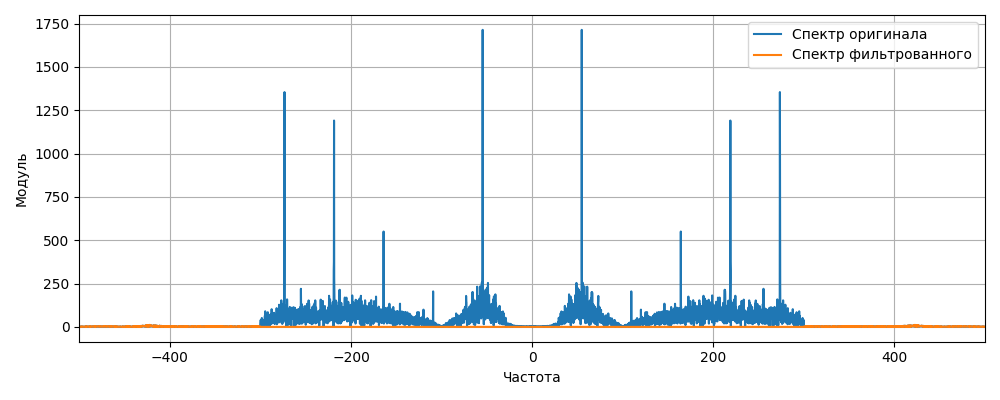
\includegraphics[width=0.8\textwidth]{src/spec_orig_filter_rec.png}
    \caption{Спектры исходного и фильтрованного сигналов}
\end{figure}
\noindent
После фильтрации видно, что:
\begin{itemize}
    \item Низкочастотные компоненты ниже $300$ Гц полностью обнулены.
    \item Основная энергия сигнала сосредоточена в голосовом диапазоне, что и позволяет лучше различать речь.
\end{itemize}
\noindent Стоит отметить, что при прослушивании фильтрованного файла голос стал чётче. Однако в ходе выполнения задания я подбирал оптимальные параметры фильтрации опытным путем. При малом диапозоне частот голос искажался: менялся тембр речи или снижалась разборчивость. Итоговый вариант вы также можете найти в \href{https://drive.google.com/drive/folders/1fi6P5S0JTVP9--mFtsujHoE6mchsh4uM?usp=sharing}{облаке}.  

Следовательно, можно сделать вывод, что слишком <<агрессивное>> вырезание частот может ухудшить качество речи, поэтому при восстановлении исходных сигналов стоит использовать более <<гибкие>> фильтры.
\end{document}